\documentclass[a4paper, 11pt]{article}
\usepackage{a4wide}
\usepackage[ngerman,english]{babel}
\usepackage[T1]{fontenc}
\usepackage[utf8]{inputenc}
\usepackage{times}
\usepackage{ifthen}
%\usepackage{bibgerm}
%\usepackage[citestyle=alphabetic,bibstyle=authortitle,backend=bibtex]{biblatex}
\usepackage[sorting=none,backend=bibtex]{biblatex}
\addbibresource{bib.bib}

\usepackage{graphicx}
\graphicspath{{./images/}}
\DeclareGraphicsExtensions{.pdf,.jpeg,.png,.svg}
\usepackage{hyperref}
\usepackage{movie15}
\usepackage{fixltx2e}
\usepackage{amsmath}
\usepackage{amssymb}
\usepackage{nccmath}
\usepackage{csquotes}

\usepackage{color}
\usepackage{graphicx}
\usepackage{blindtext}
\usepackage{color}
\topmargin 0cm \textheight 23cm \parindent0cm

% ---------------------------------------------
%	Commands definition
% ---------------------------------------------
\newcommand{\R}{\mathbb{R}}

\newcommand{\myName}{Kandhasamy Rajasekaran}
\newcommand{\emailID}{kandhasamy@uni-koblenz.de}
\newcommand{\matriculationID}{216100855}

\newcommand{\Title}{Fake news classification through Wikipedia using recurrent neural networks}
\newcommand{\StartDate}{01-Aug-2018}
\newcommand{\EndDate}{31-Jan-2018}
\newcommand{\subject}{Institute for Web Science and Technologies}
\newcommand{\expert}{Prof. Dr. Steffen Staab}%inkl. Titel
\newcommand{\supervisor}{Dr. Chandan Kumar} %inkl. Titel
\newcommand{\secondSupervisor}{Lukas Schmelzeisen} %inkl. Titel
\newcommand{\type}{Master Thesis}
\begin{document}
% ---------------------------------------------
%	Title
% ---------------------------------------------
\selectlanguage{ngerman}
Universit\"{a}t Koblenz - Landau \hfill \today

Department f\"{u}r Informatik,

\subject{}

\expert{}

\supervisor{}

\secondSupervisor{}

\begin{center}
	\large{\bf \type{}  \myName{}}

	\vspace*{0.5cm}

	\large{\bf \Title}
\end{center}

\setlength{\parskip}{1.5ex plus0.5ex minus 0.5ex}
% -----------------------------------------------------------------------------
%	Content
% -----------------------------------------------------------------------------
\selectlanguage{english}
%\begin{abstract}
%\frenchspacing
%\noindent
%The unprecedented growth in production and dissemination of information leads to an unprecedented growth in production and dissemination of fake news. Fake news hinders the society from progress by deterring the pursuit of true information. It is very essential to have a mechanism to detect and control fake news. Several attempts have been made which uses platform specific features, collaborative efforts of domain experts to control fake news. This research work will use wikipedia as a ground reality and cross check claims automatically. Recurrent neural networks will be used to understand wikipedia along with multiple novel ways to build false news. The performance of different configurations of neural networks will be analyzed and benchmarked against each other.
%\end{abstract}
% -----------------------------------------------------------------------------
\section{Introduction}
\frenchspacing

%Fake news - definition(Citation?) and prevalence
According to Lazer et al. \parencite{Lazer1094}, fake news is a false information, constructed intentionally (disinformation) or unintentionally (misinformation) where the publishers do not have rigorous news media editorial norms for making sure of its accuracy and credibility. The focus of this master thesis is to classify a claim as true or fake news by using Wikipedia as ground truth. In this thesis, different approaches will be used to model the fake news classification process using Wikipedia.

Fake news is prevalent, as can be seen by a research study from Allcot and Gentzkow \parencite{Allcott2017}, which states that "the average American adult saw on the order of one or perhaps several fake news stories in the months around the election, with just over half of those who recalled seeing them believing them". A large-scale empirical study with twitter dataset by Vosoughi et al. \parencite{Vosoughi1146}, reveals that fake news spread longer, faster, deeper and broader than legitimate news. It also reveals that the effects of fake news are more prominent in a political context than news about terrorism, natural disaster, science, and other domains.

%Fake news detection template - Compare against reliable source of information - that is the way to detect it, experts from each domain give their views and a consolidated decision (Citation?) Systems such as factcheck, snopes etc How they do it as against the rate at which fake news is generated?. %Manual correction is not possible. Web has seen an unprecedented growth. It is important to have automated means. (Citation?)
Most often fake news is detected by people and organizations through their common sense. There are many facts checking websites such as snopes.com, factcheck.org, politifact.com, etc., which use collaborative effort of domain experts. In these websites, each news article is tagged with a fact meter by domain experts to quantify its authenticity. The main strategy to handle fake news is to check against a reliable source of information and classify its integrity. This process works under the assumption that domain experts have good knowledge on the subject of news. Although this method helps in classifying fake news effectively, since it requires manual effort, it is expensive and unscalable to all domains. \color{red}citation pending - Also, the news articles that are checked by this manual process is very less in comparison to the rate at which the information is produced because of many social networks, blogging sites, etc.\color{black}

%Wikipedia - say 1 or 2 sentences about it being a source of information - different subject matters - wide coverage. Frequency of updates (Citation?). About the reliability of source of information in wikipedia (Citation?) - Wikipedia is peer reviewed as against the newspaper
Wikipedia is a free online encyclopedia available in more than 300 languages with a principle that anyone can edit \parencite{Wales2005}. According to Alexa\footnote{https://www.alexa.com} and SimilarWeb\footnote{https://www.similarweb.com}, Wikipedia is considered to be the fifth most popular website. The English Wikipedia\footnote{https://en.wikipedia.org/wiki/English\_Wikipedia} is the largest among all language editions of Wikipedia and it consists of more than 5 million articles. Also, the frequency of updates in the English Wikipedia is very high and it is approximately equal to 10 updates per second and 600 articles per day. The articles of Wikipedia are grouped into categories such as history, music, sports, etc., based on the main theme of its content. According to a research by Halavais et al. \parencite{Halavais2008}, it is estimated that categories that constitute at least 5\% of total articles in the English Wikipedia are music, history, geography, philosophy, science, technology, and literature. Also, it is found that, for all categories, the average size of an article is at least 20 kilobytes (excluding images) and the average edits of an article are at least 8. Thus, these results show that the breadth and depth of information in the English Wikipedia is substantial. Although it can be edited by anyone, an investigation carried out by Nature\footnote{https://www.nature.com}, reveals that the quality of content is similar to another established encyclopedia such as Britannica\footnote{https://www.britannica.com/} \parencite{Wales2005}. It has been shown that, although there are malicious users in Wikipedia, the community and its culture ensures most of the high impactful errors are rectified very quickly \parencite{Priedhorsky2007}. Thus, we hypothesize that the English Wikipedia can be used as a proxy for a reliable source of information since most of its content is true. \color{red}It is true that we are dealing only with the english language edition and Wikipedia does not reflect current affairs which is a crucial factor for considering it to cross check fake news since most of the fake news are based on current affairs. \color{black}

%Fake news detection using wikipedia as a ground reality (Attempt in Master thesis)
In this master thesis, the English Wikipedia will be considered as a ground reality or as a source of experts opinion and this knowledge will be used to cross-check claims automatically. The presence or absence of a claim in the English Wikipedia will be used as a proxy for classifying that claim as true or fake. Specifically, deep learning \parencite{Goodfellow2016} will be used to build different models for classifying fake news efficiently. Some of the models will take both claim and context information about claim as inputs. This context information will either be extracted from the English Wikipedia or derived sources like DBpedia or Wikidata. We also hypothesize that a model trained using both input and relevant context information will perform better as a fake news classifier than the model trained only with input. Different representations of context information will be experimented and evaluated based on how well it classifies fake news.

Section 2 will show a brief summary of different research about fake news classification using semantics and platform based approaches. Section 3 will introduce the required deep learning background to build fake news classifiers. Section 4 will explain the architecture of proposed system and the overall approach to be taken in this thesis. Section 5 will discuss different methods for evaluating the proposed fake news classifiers.
% ----------------------------------------------------------------------------
\section{Related work}

% FIND PAPERS FOR FOLLOWING
% Manual method for fake news - people checking sources manually in politfact, factcheck etc
% Platform based methods - manual/semi automated /automated feature engineering efforts
% Checking the authenticity semantically - using RDF, wikipedia

There has been much effort to detect fake news in microblogging platforms such as Twitter\footnote{https://twitter.com/}. Most of these works \parencite{Liu2015, Ma2015} classify a microblog as truth or fake by using platform/user-specific information such as how popular the post is, the credibility of the user who shared it, diffusion patterns, etc. Zhao, et al. \parencite{Zhao2015} have used cue terms such as \enquote{not true}, \enquote{unconfirmed} etc., in retweets or comments to detect fake news. The reasoning in their approach is that when people are exposed to fake news they will comment or retweet with such words as a response to the post. Other studies focused on using temporal characteristics of fake news during the spread. Kwon et al. \parencite{Kwon2013} used tweet volume in time series and Ma et al. \parencite{Ma2015} measured variations of social context features over time. 

However, the mentioned works only used comparatively small datasets. Wang \parencite{Wang2017} curated a dataset consisting of approximately 13,000 short statements by mining politfact.com covering a decade of information. In this approach, six machine learning models have been built ranging from logistic regression to a convolutional neural network. Along with the text data, metadata such as the speaker, subject, speaker history are also included. The convolutional neural network model used to capture surface level linguistics along with metadata performed better than other models.

Jing Ma et al. \parencite{Ma} efforts have been focused on building a recurrent neural network (RNN) to detect rumors from microblogs such as Twitter and Weibo\footnote{https://www.weibo.com} effectively. The training dataset is obtained by using keywords from fake and true news of debunking services such as Snopes\footnote{https://www.snopes.com/} and the Sina community management center\footnote{https://www.sina.com.cn/}. These keywords are used in search APIs of microblogging platforms and the found microblogs are labeled as true or fake, respectively. The social context information of a post and all its relevant posts such as comments or retweets are modeled as a variable-length time series. RNNs with different configurations are used to capture textual representations and the temporal patterns associated with those posts. An accuracy of at least 80\% was achieved by architectures using RNNs on both datasets. This method avoids handcrafted feature engineering efforts which are biased and time-consuming by only considering the text of posts. It produced better results with datasets from Twitter and Sina Weibo than all of the traditional machine learning methods it was compared against. RNNs with two layers of GRU captured long distance dependencies very well and achieved 88\% and 91\% accuracy on twitter and weibo dataset respectively. An accuracy of more than 80\% was achieved with a training time of 12 hours, whereas the average time taken for a single fake news item by debunking services were more than 50 hours.

However, the mentioned work by Jing Ma et al. is only for microblogging platforms. And also the features specified in one platform will be different from another and it is not guaranteed that this methodology will give the same results for the same news in two different platforms. The semantics of the tweets are not used and if used then it might improve the chance of achieving same results across platforms.

Ciampaglia et al. \parencite{Ciampaglia2015} used DBpedia\footnote{https://wiki.dbpedia.org/}, a knowledge graph, for checking whether a given information is factual or not. DBPedia datasets represent infobox section in Wikipedia. Therefore, it contains only non-controversial and factual information because it stems from human collaboration. Their methodology formulates the problem of checking facts into a network analysis problem which is finding the shortest path between nodes (subject and object of a sentence) in a graph. The aggregated generalities of nodes along a path in a weighted undirected graph are used as a metric for measuring the authenticity of information. The more elements are generic; the weaker the truthfulness is.  The genericness of a node is obtained by the degree of that node, that is the number of nodes connected to that node. The truthfulness of the information is improved if there exists at least one path from subject to an object with non-generic nodes. This approach exploits the indirect connections to a great extent with distance constraints in a knowledge graph. The approach was evaluated against four datasets: directors and their movies, US presidents and their spouses, US states and their capital and countries and their capital. The approach assigns better scores to true statements than the false statements with probabilities 0.95, 0.98, 0.61 and 0.95 for director, spouse, US capital and world capital datasets, respectively.

The mentioned work by Ciampaglia et al. is a good step towards an automated fact checker system using only the semantics of data. However, the methodology implemented is primitive and can work only for statements which have a simple relationship between the subject and object. We should also say that the evaluation approach used simple datasets and it is not really fake news. blah blah

%limitations
%-----------
%1)primitive - the complexity of news dealt with is very primitive. Current fake news are very complex and subtle when it comes to the ambiquities
%2) Semantic proximity methodology is simple and primitive


%But it is a good initial step towards an automated fact checker system.


%What improvements are we going to bring?
%----------------------------------------
%1) Ours would also be primitive :-) May be slightly better :-)
%2) Frequency of conversion of wikipedia content into DBPedia is lesser ??
%3) DBPedia does not cover the whole of wikipedia ???? 

%Things to do:
%-------------
%1) Find the answers for above questions
%2) Get the dataset that we can use?
%3) Try to look for a demo of this system

  

%Attempts made to figure out fake news in the past
%Manually curated facts dataset
%If there are any automatic ones
%It would be nice to see a forum/wiki (I hope not wikipedia :-)) being used and the methodology that have been used

%Research by Filippo Menczer - uses the DBPedia which is a structured wikipedia and use it to cross check claims
%https://www.mendeley.com/viewer/?fileId=631c34ce-5e90-722b-2974-6d71a44ad9ef&documentId=4c0051e0-64fb-3e10-959e-ac8046c9002b

%Twitter has been used - 
%https://885d47c6-a-62cb3a1a-s-sites.googlegroups.com/site/iswgao/home/ijcai16.pdf?attachauth=ANoY7cq8X9N6sGSW7wLfGloRItBkaFO1a2ELhv4s2rWN8VXGMbTwuTjUh_uGRA5vslyvOT1UDNx5wpxCWdZLNeaBcqvLO9N3dfgJfhphfDNv3pZh1P69EgHWJZeg2wGjSGDI-bhBo4VHDDwFqqM-JDoNCigNHEoTK3zDi4Dn6mGIAMcmOUfs6KrEBdAk0QUpJWPmrARCylfQe41FkVkZ0Hkpo2w-akFauQ%3D%3D&attredirects=0

%Social networks - using usage patterns in social networks- 
%https://www.mendeley.com/viewer/?fileId=6e662e87-8846-c9c3-5a3b-505f835bd89b&documentId=f238c7a0-21a1-3cab-9ed4-1c864aa0011c

% ----------------------------------------------------------------------------
\section{Background Study}

In this thesis, the proposed system will use many neural network architectures to classify fake news. The required information to understand different components of the proposed system is explained briefly in this section. Every sentence of Wikipedia would be fed and the system will be trained to remember it. Several other techniques will be tried to improve the efficiency in learning. One of it is extracting information related to an input sentence, inputting it along with sentence and training the system. This is achieved by using attention mechanism in neural networks.

\subsection{Neural networks and its components}

Recently, neural networks have become the most popular approach for building machine learning systems. Neural networks compose many interconnected, fundamental, functional units called neurons. Each neuron in the network takes in multiple scalar inputs and multiplies each input by a weight and then sums them, adds the result with a bias, applies a non-linear function at the end, which gives out a scalar output. There are different architectures of neural networks which vary mostly in how the neurons are connected to each other and how the weights are managed. 

Feed-forward neural networks \parencite{Svozil1997} can have multiple layers and each neuron in one layer is connected with every other neuron in the subsequent layer as given in the Figure \ref{fig:Feed forward neural network}

\begin{figure}[htpb]
    \centering
    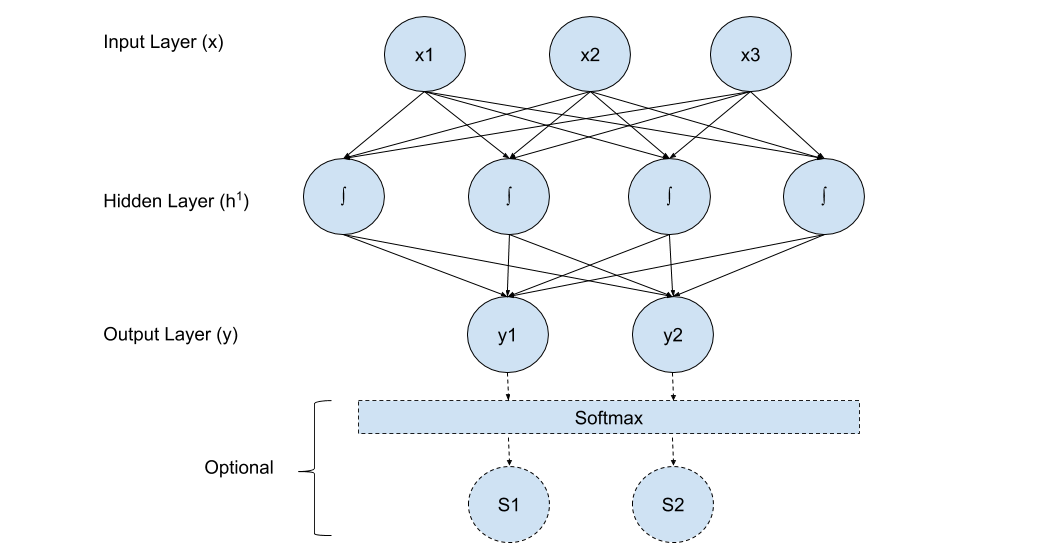
\includegraphics[width=\textwidth,height=8cm,keepaspectratio=true]
    {feed-forward-neural-network.png}
    \caption{
        A Feed-Forward neural network.
    }
    \label{fig:Feed forward neural network}
\end{figure}

There are 4 layers in figure \ref{fig:Feed forward neural network}. Each circle is a neuron with incoming lines as inputs and outgoing lines as outputs to the next layer. Each line carries a weight and the input layer has no weights since it has no incoming lines. The input layer consists of 3 neurons and the extracted features of raw data will be sent through these neurons. The first hidden layer consists of 4 neurons, of which each neuron takes 3 inputs from input layer. Each input to the neuron in first hidden layer is multiplied by a unique weight variable and added together.  Finally, the output is added with a bias variable and will be passed to a non-linear activation function as shown in equation \ref{equ: feed forward hidden layer}. The same process is carried out for the second hidden layer except that it has 3 neurons and each neuron will take 4 inputs from the first hidden layer. The output layer consists of 2 neurons and each will take 3 inputs from second hidden layer as shown in equation \ref{equ: feed forward output layer}.

\begin{equation} \label{equ: feed forward hidden layer}
h^1 = g^1(xW^1 + b^1)
\end{equation}

\begin{equation}
h^2 = g^2(h^1W^2 + b^2)
\end{equation}

\begin{equation} \label{equ: feed forward output layer}
\mathrm{NN_{MLP2}}(x) = y = g^3(h^2W^3 + b^3)
\end{equation}
\begin{align*}
x \in \mathbb{R}^{d_{in}}, y \in \mathbb{R}^{d_{out}} \\
W^1 \in \mathbb{R}^{d_{in} \times d_1}, b^1 \in \mathbb{R}^{d_1}, h1 \in \mathbb{R}^{d_{1}} \\
W^2 \in \mathbb{R}^{d_1 \times d_2}, b^2 \in \mathbb{R}^{d_2}, h2 \in \mathbb{R}^{d_{2}}\\
W^3 \in \mathbb{R}^{d_2 \times d_\mathrm{out}}, b^3 \in \mathbb{R}^{d_{out}}
\end{align*}

Here $\mathbf{W^1, W^2, W^3}$,  and $\mathbf{b^1}$, $\mathbf{b^2}$ and $\mathbf{b^3}$ are matrices and bias vectors for first, second and third linear transforms, respectively. The functions $g^1$, $g^2$ and $g^3$ are activation functions and they are almost always non-linear. With respect to figure~\ref{fig:Feed forward neural network}, the values of $d_\mathrm{in}$, $d_{1}$, $d_{2}$ and $d_\mathrm{out}$ are 3, 4, 3, and 2, respectively. 

The activation functions help the neural network models to approximate any nonlinear function. Different activation functions pose different advantages. Some popular activation functions are sigmoid, hyperbolic tangent and rectifiers \parencite{Goldberg2016}:

\begin{enumerate}

\item The sigmoid activation function is a S-shaped function which transforms any value into the range between $0$ and $1$.  
\begin{align*}
\sigma (x) = \frac{1}{1 + e^{-x}}
\end{align*}

\item The hyperbolic tangent function is also a S-shaped function, but it transforms any value into the range between $-1$ and $1$.
\begin{align*}
\tanh (x) = \frac{e^{2x}-1}{e^{2x}+1}
\end{align*}

\item The rectifier activation function clips values lesser than $0$
\begin{align*}
\mathrm{ReLU}(x) = \mathrm{max}(0,x)
\end{align*}

\end{enumerate}

The sigmoid activation function is not used in internal layers of neural networks since other functions have been giving better results empirically. The rectifier activation function is commonly used since it performs faster and better than sigmoid and hyperbolic tangent functions. Instead of an activation function, the function in output layer $g^3$ can be a transformation function such as softmax to convert values to represent a discrete probability distribution. Each of the converted values will be between $0$ and $1$ and sum of all of them will be $1$.

\begin{align*}
y = \begin{bmatrix} y_1 & y_2 & \dots & y_k \end{bmatrix} \\
s_i = \mathrm{softmax(y_i)} = \frac{e^{y_i}}{(\sum_{j=1}^ke^{y_j})}
\end{align*}

\subsection{Training a neural network}

Training is an essential part of learning and like many supervised algorithms, a loss function is used to compute the error for the predicted output against the actual output. The gradient of the errors is calculated with respect to each weight and bias variable by propagating backward using chain rule of differentiation. The values of the weights and bias are adjusted with respect to the gradient and a learning parameter. Typically a random batch of inputs is selected and a forward pass is carried out which involves multiplying weights, adding bias and applying an activation function to predict outputs. The average loss is computed for that batch and the parameters are adjusted accordingly. This optimization technique is called stochastic gradient descent \parencite{Bottou2012}. A number of extensions exists, such as Nesterov Momentum \parencite{Sutskever2013} or AdaGrad \parencite{Duchi2011}. Some loss functions that exist are hinge loss (binary and multiclass), log loss and categorical cross-entropy loss \parencite{Goldberg2016}. 

%\begin{align*}
%L_{hinge(binary)}(\hat{y},y) = max(0,1-y.\hat{y})
%\end{align*}

The categorical cross-entropy loss is used when predicted output refers to a probability distribution. This is typically achieved by using a softmax activation function in the output layer. Let $y = y^{1}, y^{2}, \dots, y^{n}$ be representing the target multinomial distribution over the labels $1,2,\dots,n$ and let $ \hat{y} = \hat{y}_{1},\hat{y}_{2},\dots,\hat{y}_{n}$ be the network's output which is transformed by a softmax function. The categorical cross-entropy loss measures the difference between the true label distribution $y$ and the predicted label distribution $\hat{y}$. 
\begin{align*}
L_\mathrm{cross-entropy}(\hat{y},y) = -\sum_iy_i \cdot \log(\hat{y_i})
\end{align*}

For hard classification, $y$ is a one-hot vector representing the true class. Here $t$ is the correct class assignment. Training will attempt to set the correct class $t$ to 1 which inturn will decrease the other class assignment to 0.
\begin{align*}
L_{\mathrm{cross-entropy(hard classification)}}(\hat{y},y) = -\log(\hat{y_t})
\end{align*}

The overfitting in neural networks will cause the trained system to perform well only for trained data but not on the test data. This can be minimized by using regularization techniques such as $L_2$ regularization and dropout \parencite{Hinton2012}. $L_2$ regularization works by adding a penalty term equal to sum of the squares of all the parameters in the network to the loss function which is being minimized. Dropout, instead, works by randomly ignoring half of the neurons in every layer and corrects the error only using the parameters of other half of neurons. This helps to prevent the network from relying on only specific weights.

\subsection{Neural networks for text data}

In case of text data, the input is sequential and of unknown length, where the ordering of words is important. Techniques such as continuous bag of words \parencite{DBLP:journals/corr/abs-1301-3781} can be used with feed-forward networks to convert sequential input into fixed length vectors but it will discard the order of words. Convolutional neural networks (CNN) \parencite{Bengio1997} are good at capturing the local characteristics of data irrespective of its position. In this, a nonlinear function is applied to every $k$-word sliding window and captures the important characteristics of the word in that window. All the important characteristics from each window are combined by either taking maximum or average value from each window. This captures the important characteristics of a sentence irrespective of its location. However, because of the nature of CNNs they fail to recognize patterns that are far apart in the sequence.

Recurrent neural networks (RNN) accept sequential inputs and are often able to extract patterns over long distances \parencite{Elman}. A RNN takes input as an ordered list of input vectors $\mathrm{\mathbf{x_1},\dots,\mathbf{x_n}}$ with initial state vector $\mathbf{h_0}$ and returns an ordered list of state vectors $\mathrm{\mathbf{h_1},\dots,\mathbf{h_n}}$ as well as an ordered list of output vectors $\mathrm{\mathbf{o_1},\dots,\mathbf{o_n}}$. At time step $t$, a RNN takes as input a state vector $\mathbf{h_{t-1}}$, an input vector $\mathbf{x_{t}}$ and outputs a new state vector $\mathbf{h_{t}}$ as shown in figure \ref{fig:A basic RNN architecture}. The outputted state vector is used as input state vector at the next time step. The same weights for input, state, and output vectors are used in each time step.  

%RNN - architecture, how does it support the sequence, (Elman, 1990) 
%Back Propagation through time (BPTT) - (Werbos, 1990) \parencite{Werbos1990}
%Long distance dependencies - LSTM and GRU (Hochreiter and Schmidhuber 1997) and (Cho et al.)
%(did not find the citation for GRU) \parencite{Hochreiter1997}
%Recursive Neural Networks - for syntactic structure (trees ) (pollack 1990; socher, manning and ng 2010) \parencite{Pollack1990} \parencite{Socher}

\begin{figure}[htpb!]
    \centering
    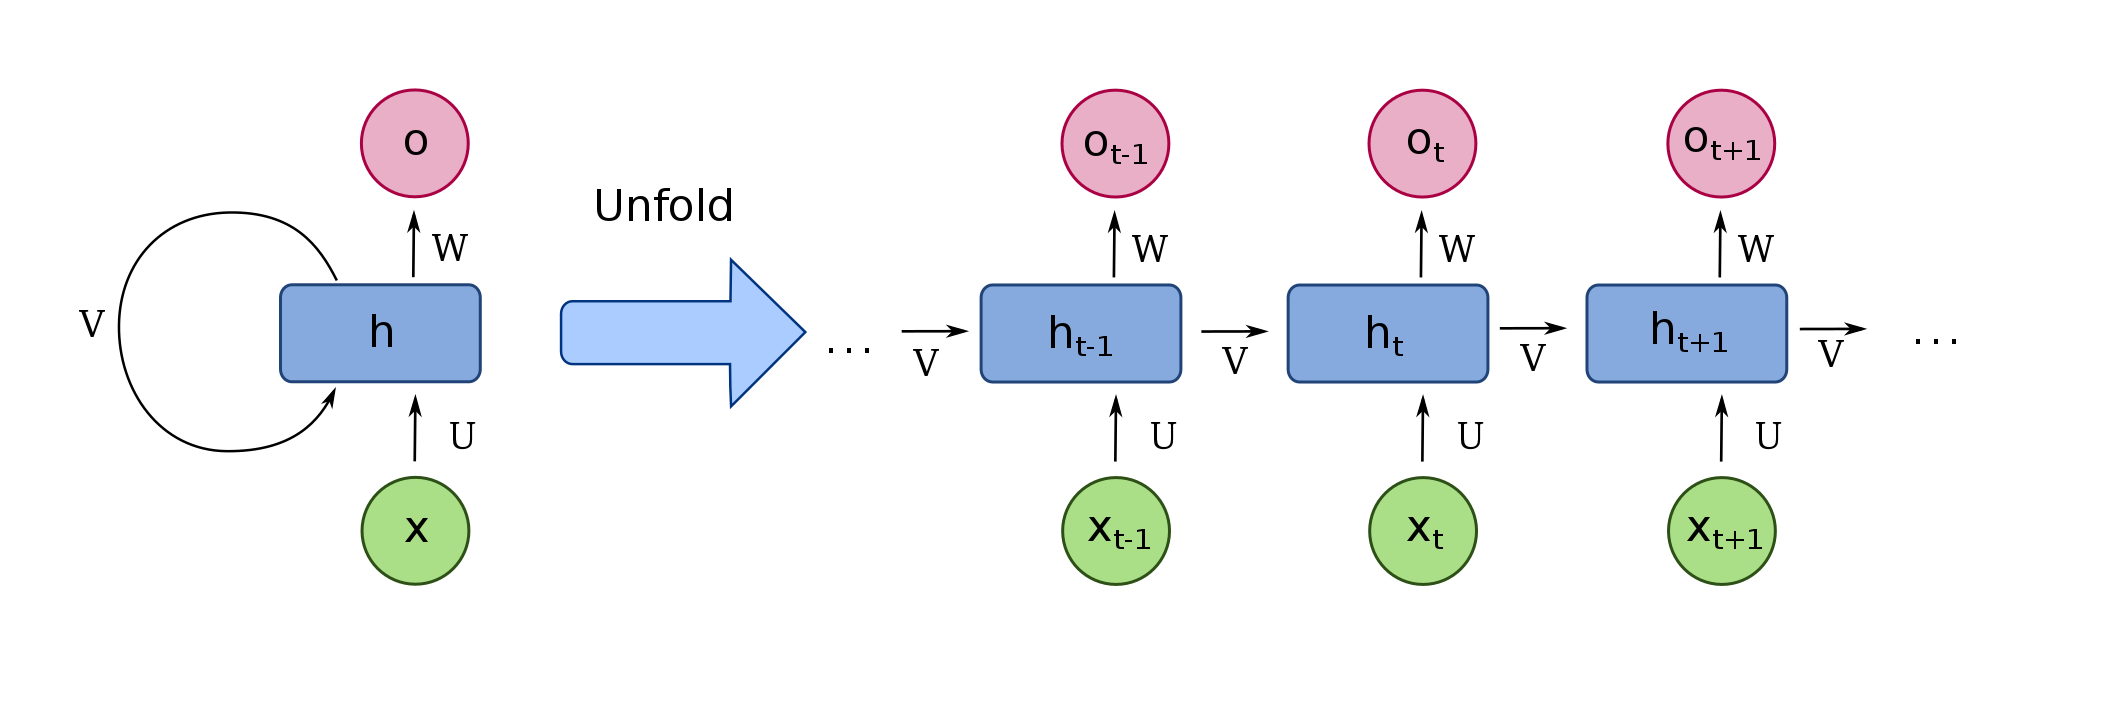
\includegraphics[width=\textwidth,height=6cm,keepaspectratio=true]
    {Recurrent_neural_network_unfold.png}
    \caption{
        A basic example of RNN architecture \parencite{WikipediaEN_RNN_unfold}.
    }
    \label{fig:A basic RNN architecture}
\end{figure}

\begin{align*}
\mathrm{RNN}(h_0,x_{1:n}) = h_{1:n}, o_{1:n} \\
h_i = g^1(h_{i-1}V + x_iU + b^1) \\
o_i = g^2(h_iW + b^2) 
\end{align*}

\begin{align*}
x_i \in \mathbb{R}^{d_x}, U \in \mathbb{R}^{d_x \times d_h} \\
h_i \in \mathbb{R}^{d_h}, V \in \mathbb{R}^{d_h \times d_h}, b^1 \in \mathbb{R}^{d_h} \\
o_i \in \mathbb{R}^{d_o}, W \in \mathbb{R}^{d_h \times d_o}, b^2 \in \mathbb{R}^{d_o}
\end{align*}

Here the functions $g^{1}$ and $g^{2}$ are non-linear activation functions; $\mathbf{W}$, $\mathbf{V}$, and $\mathbf{U}$ are weight matrices and $\mathbf{b^{1}}$, $\mathbf{b^{2}}$ are bias vectors. 

To train a RNN, the network is unrolled for a given input sequence and the loss function is used to compute the gradient of error with respect to parameters involved in every time step by propagating backward through time. After that, the parameters are adjusted to reduce the error in prediction \parencite{Werbos1990}. While training RNNs, a common problem that especially occurs with long input sentences is that the error gradients might vanish (become too close to zero) or explode (become too large) which results in numerical instability during the backpropagation step. The gradient explosion can be handled by clipping a given gradient when it goes beyond the threshold. LSTM networks \parencite{Hochreiter1997} solve the vanishing gradient problem by introducing memory cells which are controlled by gating components. These gating components decide at each time step, what parts of the hidden state should be forgotten and what parts of new input should be included into the memory cells. These memory cells are involved in the computation of hidden states, which in turn are used to compute the output states. This technique has been shown to provide good results in practice, in capturing the dependency between words even though separated by a long distance.

%\begin{align*} \label{lstm_equation}
%s_j = R_{LSTM}(s_{j-1},x_j) = [c_j;h_j] \\
%c_j = c_{j-1} \odot f + g \odot i \\
%h_j = tanh(c_j) \odot o \\
%i = \sigma(x_jW^{xi} + h_{j-1} W^{hi}) \\
%f = \sigma(x_jW^{xf} + h_{j-1} W^{hf}) \\
%o = \sigma(x_jW^{xo} + h_{j-1} W^{ho}) \\
%g = \sigma(x_jW^{xg} + h_{j-1} W^{hg}) \\
%y_j = O_{LSTM}(s_j) = h_j \\
%s_j \in \mathbb{R}^{2.d_h},   x_i \in \mathbb{R}^{d_x},  c_j,h_j,i,f,o,g \in \mathbb{R}^d_h, \\
%W^{xo} \in \mathbb{R}^{d_x*d_h},  W^{ho} \in \mathbb{R}^{d_h*d_h}
%\end{align*}
%Here the symbol $\odot$ denotes component wise product. The LSTM uses 3 gating components such as input gate (i), forgot gate (f) and output gate (o) respectively. They contain a sigmoid function to convert the values between 0 and 1 which is used to decide how much to keep. The memory cell state c\textsubscript{j} is obtained by controlling the previous memory cell state with forgot gate and the new input state (g) with input gate. The obtained memory cell state is controlled by output gate to get the hidden state h\textsubscript{j}.

\subsection{Neural networks for improving fake news classification }

A RNN computes the state of current word $\mathbf{x_{i}}$ only based on the words in the past, i.e. $\mathrm{\mathbf{x_1},\dots,\mathbf{x_{i-1}}}$. However, the following words $\mathrm{\mathbf{x_{i+1}},\dots,\mathbf{x_{n}}}$ will also be useful in computing the hidden state regarding the current word. The Bidirectional RNN (biRNN) (Schuster and Paliwal, 1997) solves the problem by having two different RNNs. The first RNN is fed with the input sequence $\mathrm{\mathbf{x_{1}},\dots,\mathbf{x_{n}}}$ and the second RNN is fed with input sequence in reverse. The hidden state representation $\mathbf{h_{i}}$ is then composed of both the forward and backward states. Each state representation consists of the token information along with sentential context from both directions which has shown better results than classical uni-directional RNNs in practice.

The mentioned approaches take only Wikipedia sentence as an input. This can be extended further by feeding information which gives context about the input sentence. This extra information might enable the system to perform efficiently in classifying whether a news item is fake or not. Attention mechanism in neural networks is used to take two inputs and convert it into one common representation. This is done by configuring the level of attention that needs to be given to different parts of each input and combine them to form a single output. Most often the inputs will be matrices and the output will be a vector. Bidirectional RNNs can be used to convert both input and context information into matrices. The fixed output vector is then fed into a deep feed-forward neural network to predict a class. Attention mechanism with RNN gives state of the art results in many NLP applications such as Natural Language Inference \parencite{Parikh2016}, Machine Translation \parencite{Bahdanau2014} and Document classification \parencite{Yang2016}.

\section{Approach}  

The task is to build a fake news classifier using Wikipedia and cross-check claims. The input to this classifier will be a sentence representing a claim and the output from this classifier will be a binary value representing the inputted sentence as true or fake. For example, when the sentence 'Obama is a muslim' is sent as an input to classifier then the output will be a binary value '0' representing the input is fake. Similary, for the input sentence 'Obama is a christian', the classifier will output a binary value '1' representing the input is truthy. 

\subsection{Research Questions}

Through this work, the research questions that would be addressed are:
\begin{enumerate}
\item  Wikipedia is large and the proposed system may not be able to remember all the sentences. How well can we memorize or recognize sentences from Wikipedia in a neural network? This will give an understanding of the limitations of proposed system. 
\item How well Wikipedia be used for fake news detection?. Does Wikipedia contains all relevant information to detect wide spectrum of fake news? This would uncover the limitations of Wikipedia to be used as a fake news classifier. 
%How close are generated negative examples to actual fake news?
\item Since it is difficult to remember everything in Wikipedia, depending on the claim to be checked, selected portions of Wikipedia will be retrieved and used as a context. This approach will overcome the limitation of not being able to remember everything in Wikipedia to a certain extent. How good can we recognize fake news information in context data from Wikipedia?
\end{enumerate}

\subsection{Model}

Model - general architecture
Different kinds of context
Represent input + context
detailed model architecture (type of RNN, type of attention mechanism)

 A general architecture of the proposed system is as shown in figure \ref{fig:broad_architecture}

\begin{figure}[htpb]
    \centering
    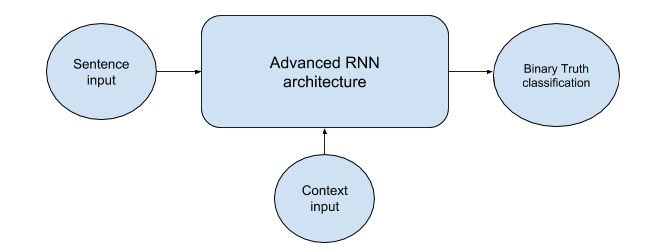
\includegraphics[width=\textwidth,height=8cm,keepaspectratio=true]
    {broad-architecture-diagram.png}
    \caption{
        Broad Architecture
    }
    \label{fig:broad_architecture}
\end{figure}

The reason behind using context input is that the RNN system would be better equipped with information to make a decision whether it is a true or fake news. And also that, the problem of fake news classification can be seen as a Natural Language Inference \parencite{Parikh2016} problem, which is about finding entailment or contradictory relationship between two sentences such as hypothesis and premise. Here, the context input is the premise and sentence input is the hypothesis. If there is an entailment between sentence input and context then it is true news otherwise false.

There are many ways by which context input can be modeled and inputted to the systems. \color{red}Extracting the context as relevant to sentence input can be challenging and a suitable information retrieval method will be selected for it.\color{black}

\begin{enumerate}
\item The context can be empty. The system would be trained to understand Wikipedia and use this information alone to make a decision.
\item Top 10 Wikipedia articles relevant to the sentence will be passed as context input. The Wikipedia articles will be long and so will increase the size of context input. The system may face long distance dependency issues and a suitable hyper-parameter selection is critical. Since both the sentence and context input are text from Wikipedia, the system might find it easy to align one with respect to other and find patterns among them. 
\item Nearly 100 triples of knowledge graph will be passed as context input. Resource Description Framework (RDF) triples of DBPedia can be used. Extracting such information from DBPedia will be relatively easier. The structure of context input will be simple and straightforward and the length of context input will be shorter than using Wikipedia articles.  
\item Information such as parts of speech, named entity and dependency graph of a sentence will be passed as context input. These metadata will bring more clarity about the sentence structure, which will help the system to extract patterns efficiently. 
\end{enumerate}

A detailed architecture of an advanced RNN system is shown in the figure \ref{fig:detailed_architecture}. The sentence input and context input will be encoded into a rich and convenient representation separately. Bidirectional RNNs can be used which will take a sequential input and convert it into a matrix. The number of rows of the matrix will be equal to number of tokens in a sentence and number of columns can be controlled. Each row in the matrix will represent a token with sentential context. Both the sentence and context representation are then combined to form an efficient common representation. The arbitrariness of both sentence and context representation will be controlled and converted into a representation of fixed length. Attention modules can be used which will figure out how much attention needs to be given to both the representations to produce a common representation. It usually takes two matrices and outputs a fixed vector. But the attention mechanism can be a pure reduction process, where it takes only one matrix and converts into a fixed vector. This can be used when the context input is empty. The predictor takes in a fixed vector as input and predicts which one of the binary class label(true or fake) is most likely the final output. A feed-forward neural network will be a good choice to be used as a predictor. 

\begin{figure}[htpb]
    \centering
    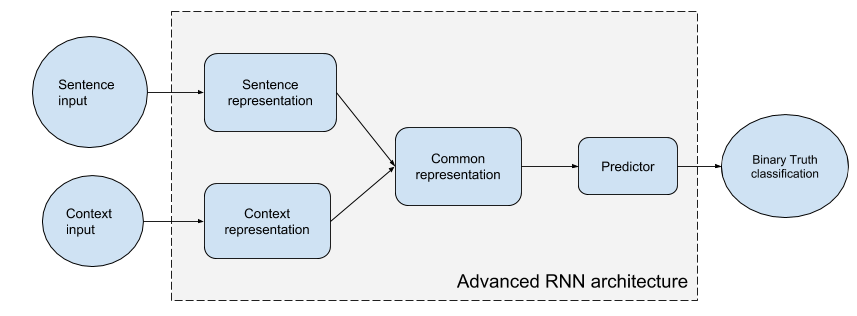
\includegraphics[width=\textwidth,height=8cm,keepaspectratio=true]
    {detailed-architecture-diagram.png}
    \caption{
        Detailed Architecture
    }
    \label{fig:detailed_architecture}
\end{figure}

\subsection{Experiments}


Experiments : 4 experiments 
Data wikipedia : sentence from wikipedia + negative examples through distortion
Data fake news : kaggle - dataset or Ciampaglia dataset

1) Training - 90 percent data wikipedia, Testing - 10 data from wikipedia
2) 100 percent Data wikipedia, Data fake news
3) 90 percent Data fake news, 10 percent data fake news
4) Data from wikipedia and fake news, data fake news

Since we use Wikipedia as a proxy for authentic information, each sentence in the Wikipedia is considered as true news. There is hardly any false news present. For training to be successful to build a good fake news detector, it should be ensured that more or less equal amount of data should be present for both true and fake news. The construction of false news is tricky and different natural language processing (NLP) methods will be used to generate false news. Spacy\footnote{https://www.spacy.io}, a python library for NLP tasks will be used for extracting parts of speech, named entity and dependency relations. Some techniques are 
\begin{enumerate}
\item Swap the words randomly in each and every sentence extracted from Wikipedia. The RNN models used will remember the sequence information and so a randomly shuffled sentence will be considered as a different sentence by the system. However, the syntax and semantics of the sentence created will be poor. This method is primitive but it will serve as a good baseline. 
\item Replace the random words picked in a sentence with a random word from the corpus. This method would retain some of the words as it is and changing only few words will bring a subtle change in sentence. This is similar to random swapping but the syntactic structure of the sentence will be preserved to some extent.
\item Replace all or randomly picked words in a sentence based on their parts of speech. In this method, all the words in the corpus will be tagged with a parts of speech label. This information will be used and randomly a word will be picked from the corpus which has the same parts of speech as the word to be replaced. This method will preserve the syntactic structure of the sentence better than the previous methods. 
\item Replace the words in each sentence with their opposites extracted from WordNet\footnote{https://wordnet.princeton.edu/}. This method will not only preserve the syntax but also likely to have right semantics. The sentence created will more likely to have a meaning which is opposite of the original sentence. 
\item Extract the dependency tree for each sentence and select an appropriate one from other sentences to replace it. The dependency relationship will contain information about which words are dependent on which other words. Replacing based on this similarity may create better examples.
\end{enumerate}

Total 80 experiments. 4 ways to create a model. 5 ways to create negative examples. and 4 ways of experiments

\subsection{Implementation}

Implementation: Tensorflow, spacy 

Recurrent neural networks will be used in this master thesis extensively since they perform well with sequential data. TensorFlow\footnote{https://www.tensorflow.org/} is a python library for building intensive numerical computation applications and deploy them in multiple platforms such as CPU and GPU. TensorFlow has built-in libraries to develop different neural network architectures. Wikipedia consists of a lot of articles; each article consists of a lot of sentences. Each sentence will be fed as input to the neural network.
---------------
An advanced RNN architecture takes in either one or two inputs such as sentence in Wikipedia and context information. The context can be empty. The system processes the input and produces a binary output representing true or fake news. The outputs would contain a probability distribution of how likely it is true or fake news.

The inputs, in general, will be pre-processed to extract tokens, remove common words such as articles, prepositions and perform lemmatization which is converting the words to its root form. Low dimensional and dense word embeddings will be used to represent the inputs instead of one hot vectors. Already available word embeddings such as Word2vec \parencite{Mikolov2013} and GloVe\footnote{https://nlp.stanford.edu/projects/glove/} will be used to represent the inputs.

The dataset will be split and used for training, validation, and testing of the system. A general rule of thumb is to divide the dataset into 60-20-20 for training, validation, and testing respectively. But if the datasets are in order of millions then it is good enough to have approximately 10000 entries each for validation and testing. The validation dataset is used to try out different hyper-parameter configurations and select the optimal values for each. The hyper-parameters of the advanced neural network system that will be configured are number of layers, learning parameter, batch size, activation functions and epoch number(number of times the training dataset should be iterated).

% Background Knowledge: Wikidata or BabelNet (knowledge graphs), http://babelfy.org/ for entity resolution

The proposed methods involve modeling the content of Wikipedia in different ways such that the system can understand it better. These procedures are completely automatic in building the training examples and none of the features will be manually crafted. The different configurations of the system along with unique methods in constructing the training data is expected to understand Wikipedia better and the fake news detection can be carried out in a platform agnostic manner. 

% ----------------------------------------------------------------------------
\section{Evaluation}

The system will be evaluated as a fake news classifier. The test data should be different from the training or validation data which is used by the system. 

\subsection{Datasets}

There are two comprehensive open datasets on fake news detection available.
\begin{enumerate}
\item  One of it is published in Kaggle\footnote{https://www.kaggle.com/mrisdal/fake-news} which consists of structured data of 13,000 rows and 20 columns. Some of the important information in this dataset are title, text and spam score. 
\item The LIAR dataset is published by Wang \parencite{Wang2017} which is mined from politifact.com and it consists of 12,836 short statements. In addition to that, it also contains information about context, labels with 6 classes and justification for the label classification. 
\end{enumerate}

The mentioned datasets might be too diverse to compare the performance of the system at the beginning. It might require training from the whole of Wikipedia. Research work from Ciampaglia et al. \parencite{Ciampaglia2015} used many simple datasets to evaluate network analysis techniques on a knowledge graph to build fake news classfier. The datasets are US politicians and their party affiliation, directors and their movies, US president and their spouses, US states and their capitals and world countries and their capitals. It also involves a dataset from Google Relation Extraction Corpus (GREC) which is about education degrees and institutional affiliations of people. These datasets will help to compare the performance of fake news classifier in specific domains of knowledge against their achieved results.

In addition to that, the system can be evaluated based on how well it is able to understand Wikipedia. We use the presence and absence of a information in Wikipedia as a proxy for labeling that information as true or fake news. So, it is good to evaluate our system based on how well it is able to classify whether a given information is present in Wikipedia or not. This is done by inputting either random sentences or the sentences taken from Wikipedia and check whether it is present or not. \color{red}If the system performs very well in this test and fails to perform well with the mentioned standard datasets for fake news classification then it might help to gain insights on how good the coverage of news in Wikipedia is. \color{black}

\subsection{Metrics}

The baseline system involves only RNN and the improvements that will be added are RNN with LSTM blocks, bidirectional RNNs, and inclusion of context input along with sentence input. The following factors are used to compare the baseline with the improved system
\begin{enumerate}
\item How good the system is able to classify the non-Wikipedia news / fake news?
\item How fast the model is build up?
\end{enumerate}

The quality of the system can be measured by metrics such as Precision, Recall, F1 measure, and Accuracy. The F1 measure is preferred since it includes both false positive and false negatives. In this master thesis, the focus is mainly on improving the accuracy of the system and the speed of the system can be improved by using good hardware.

\newpage

% ----------------------------------------------------------------------------
\section{Organizational matters}

\begin{tabbing}
Duration of work: \hspace{1.1cm} \= \StartDate{} -- \EndDate{}\\
\vspace{0.5ex}Candidate:	\> \myName{}\\
\vspace{0.5ex}E-Mail:	\> \emailID{}\\
\vspace{0.5ex}Student number: \> \matriculationID{}\\
\vspace{0.5ex}Primary supervisor: \> \expert{}\\
Supervisor: \> \supervisor{}\\
Secondary supervisor: \> \secondSupervisor{}\\
\end{tabbing}

% ----------------------------------------------------------------------------

\section{Time schedule}

\begin{itemize}
	\item Introduction and Literature: 01-May-2018 – 30-June-2018
	\item Initial phase: 01-Aug-2018 – 15-Oct-2018
	\begin{itemize}
		\item Prototyping: 01-Aug-2018 – 30-Aug-2018
		\item ML pipeline implementation: 01-Sep-2018 – 15-Sep-2018
        \item Baseline implementation: 15-Sep-2018 – 30-Sep-2018
        \item Testing and refining: 01-Oct-2018 – 15-Oct-2018
	\end{itemize}
	\item Development phase: 16-Oct-2018 – 30-Dec-2018
	\begin{itemize}
		\item RNN with different configuration: 16-Oct-2018 – 30-Oct-2018
		\item Comprehend benchmark results: 16-Oct-2018 – 30-Oct-2018
		\item Analyse and figure out improvements: 22-Oct-2018 – 30-Oct-2018
        \item Improvisation using NLP techniques: 01-Nov-2018 – 30-Nov-2018
        \item Attention mechanism implementation: 01-Dec-2018 – 30-Dec-2018
        \item Comprehend benchmark results: 16-Dec-2018 – 30-Dec-2018
	\end{itemize}
	\item Final phase: 01-Jan-2019 – 01-Feb-2019
	\begin{itemize}
	 	\item Comprehend Benchamark results: 01-Jan-2019 – 07-Jan-2019
		\item Revision: 08-Jan-2019 – 22-Jan-2019
		\item Thesis report: 01-Jan-2019 – 30-Jan-2019
	\end{itemize}
\end{itemize}

A meeting with Lukas Schmelzeisen will happen approximately once in two weeks to discuss about the progress made and set the targets and milestones for subsequent weeks. 

% ----------------------------------------------------------------------------
\newpage
\printbibliography
%\bibliography{bib.bib}
\newpage
% ----------------------------------------------------------------------------
\section{Signatures}

\vspace{3cm}
\begin{tabular}{ccc}
  --------------------------------------------------- &  & ---------------------------------------------------\\
  \myName{} &  & \expert{}  \\ \vspace{3cm}
   &  &   \\
  --------------------------------------------------- &  & ---------------------------------------------------\\
  \supervisor{} &  & \secondSupervisor{}  \\ \vspace{3cm}
   &  &   \\
\end{tabular}

\newpage
% ----------------------------------------------------------------------------
\section{Declaration of Authorship}
I hereby declare that the thesis submitted is my own unaided work. All direct or indirect sources used are acknowledged as references.

I am aware that the thesis in digital form can be examined for the use of unauthorized aid and in order to determine whether the thesis as a whole or parts incorporated in it may be deemed as plagiarism. For the comparison of my work with existing sources I agree that it shall be entered in a database where it shall also remain after examination, to enable comparison with future theses submitted. Further rights of reproduction and usage, however, are not granted here.

This paper was not previously presented to another examination board and has not been published.

\vspace{3cm}
\begin{tabular}{ccc}

  Koblenz, on \today &  &  \\
     &  & ---------------------------------------------------\\
   &  & \myName{}  \\
\end{tabular}



\end{document}









